\documentclass[hyperref=unicode]{beamer}

\usepackage[absolute,overlay]{textpos}
\usepackage{graphicx}
\usepackage{adjustbox}
\usepackage{chemfig}
\usepackage[version=4]{mhchem}
\usepackage{wrapfig}
\usepackage{multirow}
\adjustboxset*{center}
\usepackage{caption}
\usepackage{chemformula}
\usepackage{elements}

\usepackage{pgfplots}
\pgfplotsset{compat=1.18}

%dělení slov
\usepackage{ragged2e}
\let\raggedright=\RaggedRight
%konec dělení slov

\usepackage{fontspec}
\usepackage{unicode-math}

\usepackage{polyglossia}
\setdefaultlanguage{czech}

\def\uv#1{„#1“}

\usetheme[numbering=fraction]{metropolis}
%\mode<presentation>{\usetheme{Madrid}}
%\DefineNamedColor{named}{pozadi}{RGB}{200,200,200}
%\usecolortheme{crane}

%------------------------------------------------
% Fonty (LuaLaTeX nebo XeLaTeX) %------------------------------------------------
\usepackage{fontspec}
\setmainfont{Source Sans Pro}
\setsansfont{Source Sans Pro}
\setmonofont{JetBrains Mono}

%------------------------------------------------
% Grafika
%------------------------------------------------
\usepackage{graphicx}
\usepackage{booktabs}
\usepackage{multirow}
\usepackage{tikz}
\usetikzlibrary{ positioning, arrows.meta, calc, shapes.geometric }

%------------------------------------------------
% Barvy
%------------------------------------------------
\definecolor{MUblue}{HTML}{00467F}
\definecolor{MUlight}{HTML}{EAF2F8}
\definecolor{MUgreen}{HTML}{008A5E}
\setbeamercolor{frametitle}{fg=MUblue}
\setbeamercolor{title}{fg=MUblue}
\setbeamercolor{block title}{ fg=white, bg=MUlight }
\setbeamercolor{block body}{ bg=MUblue }
\setbeamercolor{alerted text}{ fg=MUgreen }

%------------------------------------------------
% Metropolis nastavení
%------------------------------------------------

\metroset{ progressbar=frametitle, sectionpage=progressbar, block=fill }

%------------------------------------------------
% Vzhled seznamů
%------------------------------------------------
\setbeamertemplate{itemize item}{\small$\blacktriangleright$} \setbeamertemplate{itemize subitem}{\tiny$\blacktriangleright$}

%------------------------------------------------
% Číslování obrázků a tabulek %------------------------------------------------

\setbeamertemplate{caption}[numbered]

% --------------------------------------------------
% Bez navigačních ikon
% --------------------------------------------------

\setbeamertemplate{navigation symbols}{}

% --------------------------------------------------
% Horní lišta se sekcí
% --------------------------------------------------

\setbeamercolor{section in head/foot}{ fg=white, bg=MUgreen } \setbeamertemplate{headline}
{ \leavevmode
	\hbox{ \begin{beamercolorbox}[ wd=\paperwidth, ht=2.8ex, dp=1.2ex, leftskip=1em ]{section in head/foot}
			\insertsectionhead

			\ifx\insertsubsectionhead\empty \else \insertsectionhead\hspace{1em}$\triangleright$\hspace{0.5em} \insertsubsectionhead \fi

		\end{beamercolorbox}
	}
}

% --------------------------------------------------
% Dolní lišta s číslováním
% --------------------------------------------------

\setbeamercolor{author in head/foot}{ fg=white, bg=MUgreen } \setbeamertemplate{footline}
{
	\leavevmode
	\hbox{
		\begin{beamercolorbox}[ wd=\paperwidth, ht=2.8ex, dp=1.2ex, rightskip=1em ]{author in head/foot}
			\hfill
			\insertframenumber/\inserttotalframenumber \end{beamercolorbox}
	}
}

\title[Crisis]
{Plasty versus lidstvo}

\subtitle{BR14OC 2. 10. 2026}
\author{Zdeněk Moravec, hugo@chemi.muni.cz \\ \adjincludegraphics[height=.5\textheight]{img/BrNOC-2026-Moravec.jpg}}
\date{}

\begin{document}
\begin{frame}
	\titlepage
\end{frame}

\section{Doba plastová}
\frame{
	\frametitle{}
	\vfill
	\begin{columns}
		\begin{column}{.65\textwidth}
			\begin{enumerate}
				\item Co jsou to plasty, mikroplasty, nanoplasty?
				\item Z čeho se plasty vyrábí?
				\item Kolik plastových výrobků máte teď u sebe?
				\item Kolik těchto výrobků je určeno pro jedno použití?
				\item Jaký podíl z těchto předmětů skončí v recyklačních kontejnerech?
				\item Jaký podíl plastů je skutečně recyklován?
				\item Co jsou to PFAS?
			\end{enumerate}
		\end{column}

		\begin{column}{.45\textwidth}
			\begin{figure}
				\adjincludegraphics[width=\textwidth]{img/Plastic_objects.jpg}
				\caption*{Výrobky z plastu.\footnote[frame]{Zdroj: \href{https://commons.wikimedia.org/wiki/File:Plastic_objects.jpg}{Cjp24/Commons}}}
			\end{figure}
		\end{column}
	\end{columns}
	\vfill
}

\section{Plasty a chemie}
\frame{
	\frametitle{}
	\vfill
	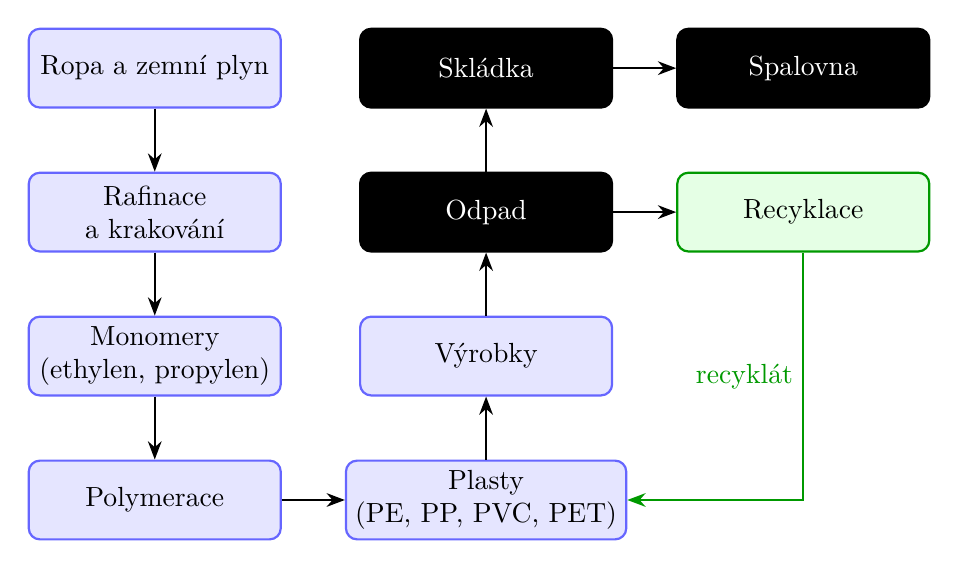
\begin{tikzpicture}[
		>=Stealth,
		node distance=0.8cm,
		block/.style={
			rectangle,
			rounded corners,
			draw=blue!60,
			fill=blue!10,
			thick,
			minimum width=3.2cm,
			minimum height=1cm,
			align=center },
			recycle/.style={
				rectangle,
				rounded corners,
				draw=green!60!black,
				fill=green!10,
				thick,
				minimum width=3.2cm,
				minimum height=1cm,
				align=center }
				]

				\node[block] (feedstock)
				{Ropa a zemní plyn};

				\node[block,below=of feedstock] (cracking)
				{Rafinace\\a krakování};

				\node[block,below=of cracking] (monomers)
				{Monomery\\(ethylen, propylen)};

				\node[block,below=of monomers] (polymer)
				{Polymerace};

				\node[block,right=of polymer] (plastics)
				{Plasty\\(PE, PP, PVC, PET)};

				\node[block,above=of plastics] (products)
				{Výrobky};

				\node[block,above=of products,
				draw=black,
				fill=black!120,
				text=white] (waste)
				{Odpad};

				\node[block,above=of waste,
				draw=black,
				fill=black!120,
				text=white] (garbage)
				{Skládka};

				\node[block,right=of garbage,
				draw=black,
				fill=black!120,
				text=white] (incinerator)
				{Spalovna};


				\node[recycle,right=of waste] (recycling)
				{Recyklace};

				\draw[->,thick] (feedstock) -- (cracking);
				\draw[->,thick] (cracking) -- (monomers);
				\draw[->,thick] (monomers) -- (polymer);
				\draw[->,thick] (polymer) -- (plastics);
				\draw[->,thick] (plastics) -- (products);
				\draw[->,thick] (products) -- (waste);
				\draw[->,thick] (waste) -- (recycling);
				\draw[->,thick] (waste) -- (garbage);
				\draw[->,thick] (garbage) -- (incinerator);
				\draw[->,thick,green!60!black] (recycling)
				|- node[pos=0.25,left]
				{recyklát} (plastics.east);
				\end{tikzpicture}
	\vfill
}

\frame{
	\frametitle{}
	\vfill
	\begin{figure}
		\adjincludegraphics[width=1.1\textwidth]{img/Plasty.png}
		\caption*{Nejpoužívanější plasty}
	\end{figure}
	\vfill
}

\section{Plasty v číslech}
\frame{
	\frametitle{}
	\vfill
	\begin{figure}
		\adjincludegraphics[width=.9\textwidth]{img/Plasty-vyroba.png}
		\caption*{Objem celosvětové roční výroby plastů v letech 1950--2019.\footnote[frame]{Zdroj: \href{https://ourworldindata.org/grapher/global-plastics-production?time=1950..2019}{Our World in Data}}}
	\end{figure}
	\vfill
}

\frame{
	\frametitle{}
	\vfill
	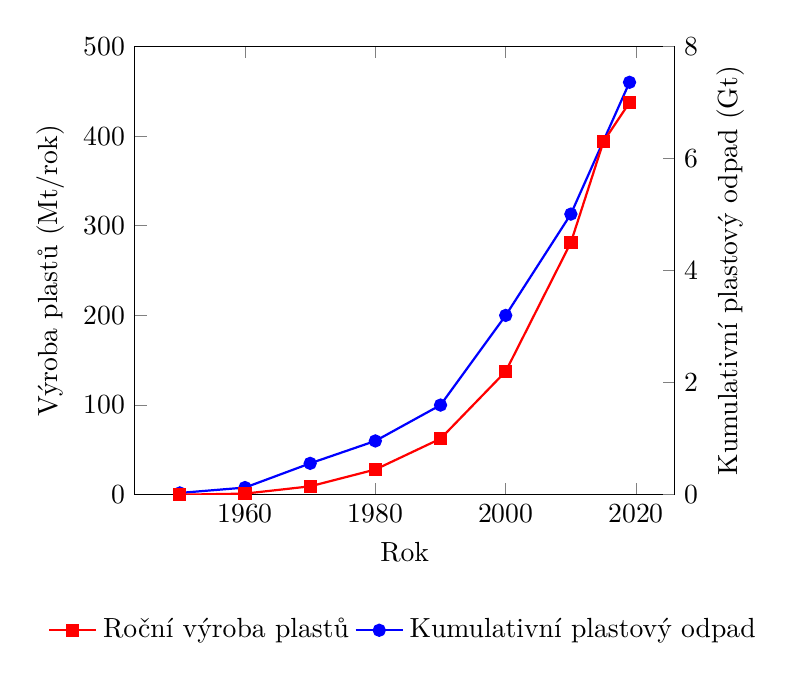
\begin{tikzpicture}
	\begin{axis}[
		axis y line*=left,
		xlabel=Rok,
		ylabel=Výroba plastů (Mt/rok),
		ymin=0,
		ymax=500,
		xticklabel style={
			/pgf/number format/1000 sep={}
		} ,
		]

		\addplot[blue,thick,mark=*]
		coordinates {
			(1950,2)
			(1960,8)
			(1970,35)
			(1980,60)
			(1990,100)
			(2000,200)
			(2010,313)
			(2019,460)
			};
		\end{axis}

		\begin{axis}[
			axis y line*=right,
			axis x line=none,
			ylabel=Kumulativní plastový odpad (Gt),
			ymin=0,
			ymax=8,
			legend style={
				at={(0.5,-0.25)},
				anchor=north,
				legend columns=2,
				fill=none,
				draw=none
			}
			]

			\addplot[red,thick,mark=square*]
			coordinates
			{
				(1950,0.0)
				(1960,0.02)
				(1970,0.15)
				(1980,0.45)
				(1990,1.0)
				(2000,2.2)
				(2010,4.5)
				(2015,6.3)
				(2019,7.0)
			};

			\addlegendimage{blue,thick,mark=*}
			\addlegendentry{Roční výroba plastů} \addlegendimage{red,thick,mark=square*} \addlegendentry{Kumulativní plastový odpad}
		\end{axis}
	\end{tikzpicture}
	\vfill
}

\section{Plasty v našem životě}
\frame{
	\frametitle{}
	\vfill
	\begin{columns}
		\begin{column}{.4\textwidth}
			\textbf{Proč jsou pro nás plasty tak důležité?}
			\vspace{5mm}

			Jsou:
			\begin{itemize}
				\item Lehké
				\item Levné
				\item Odolné
				\item Snadno tvarovatelné
			\end{itemize}
		\end{column}

		\begin{column}{.65\textwidth}
			\begin{figure}
				\adjincludegraphics[width=\textwidth]{img/Plastic_objects.jpg}
				\caption*{Plastové výrobky.\footnote[frame]{Zdroj: \href{https://commons.wikimedia.org/wiki/File:Plastic_objects.jpg}{Cjp24/Commons}}}
			\end{figure}
		\end{column}
	\end{columns}
	\vfill
}

\frame{
	\frametitle{}
	\vfill
	\begin{columns}
		\begin{column}{.3\textwidth}
			\textbf{Co se s plasty děje po jejich použití?}
			\vspace{5mm}

			\begin{itemize}
				\item Skládka
				\item Spalovna
				\item Recyklace
			\end{itemize}
		\end{column}

		\begin{column}{.75\textwidth}
			\begin{figure}
				\adjincludegraphics[width=\textwidth]{img/Pollution_plastique_2.jpg}
				\caption*{Plastový odpad.\footnote[frame]{Zdroj: \href{https://commons.wikimedia.org/wiki/File:Pollution_plastique_2.jpg}{Mouenthias/Commons}}}
			\end{figure}
		\end{column}
	\end{columns}
	\vfill
}

\frame{
	\frametitle{}
	\vfill
	\begin{figure}
		\adjincludegraphics[width=\textwidth]{img/PET-lahev.png}
		\caption*{Životní cyklus PET láhve.}
	\end{figure}
	\vfill
}

\frame{
	\frametitle{}
	\vfill
	\begin{itemize}
		\item Bohužel, většina plastového odpadu neskončí ve spalovně nebo recyklačním zařízení.
		\item Podle statistik bylo v roce 2018:\footnote[frame]{\href{https://css.umich.edu/publications/factsheets/material-resources/plastic-waste-factsheet}{Plastic Waste Factsheet}}
		\begin{itemize}
			\item spáleno 16~\% odpadu
			\item recyklováno jen 9~\% odpadu
			\item zbytek, tzn. 76~\%, plastového odpadu skončí na skládkách nebo ve volné přírodě
		\end{itemize}
		\item Šance na recyklaci se zvyšuje vyhozením plastů do žlutého kontejneru.
		\item V Brně bylo v roce 2023 sebráno asi 3777 tun plastového odpadu.
		\begin{itemize}
			\item recyklováno bylo 68~\%, tj. asi 2568 tun odpadu
			\item spáleno bylo 32~\%, tj. asi 1209 tun odpadu
		\end{itemize}
	\end{itemize}
	\vfill
}

\section{Recyklace plastů}
\frame{
	\frametitle{}
	\vfill
	\textbf{Životní cesta PET láhve:}

	\centering

	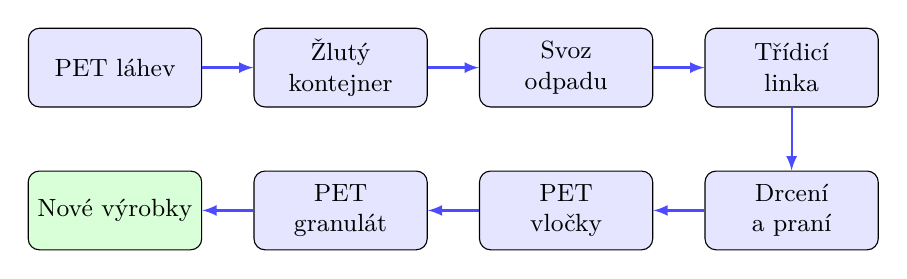
\begin{tikzpicture}[
		>=latex,
		node distance=0.65cm,
		process/.style={
			draw,
			rounded corners,
			fill=blue!10,
			minimum width=2.2cm,
			minimum height=1cm,
			align=center,
			font=\small
			},
			arrow/.style={ ->, thick, blue!70 }
			]

			\node[process] (a) {PET láhev};
			\node[process,right=of a] (b) {Žlutý\\kontejner};
			\node[process,right=of b] (c) {Svoz\\odpadu};
			\node[process,right=of c] (d) {Třídicí\\linka};
			\node[process,below=0.8cm of d] (e) {Drcení\\a praní};
			\node[process,left=of e] (f) {PET\\vločky};
			\node[process,left=of f] (g) {PET\\granulát};
			\node[process,left=of g,fill=green!15] (h) {Nové výrobky};

			\draw[arrow] (a) -- (b);
			\draw[arrow] (b) -- (c);
			\draw[arrow] (c) -- (d);
			\draw[arrow] (d) -- (e);
			\draw[arrow] (e) -- (f);
			\draw[arrow] (f) -- (g);
			\draw[arrow] (g) -- (h);
		\end{tikzpicture}

		\begin{block}{Co může vzniknout z recyklovaného PET?}
			Nové lahve, textilní vlákna (fleece), fólie, pásky nebo technické díly.
		\end{block}

		\textbf{Tímto postupem nelze plasty recyklovat donekonečna, protože dochází k jejich postupné degradaci.}
	\vfill
}

\frame{
	\frametitle{}
	\vfill
	\textbf{Schéma automatické třídící linky:}

	\centering

	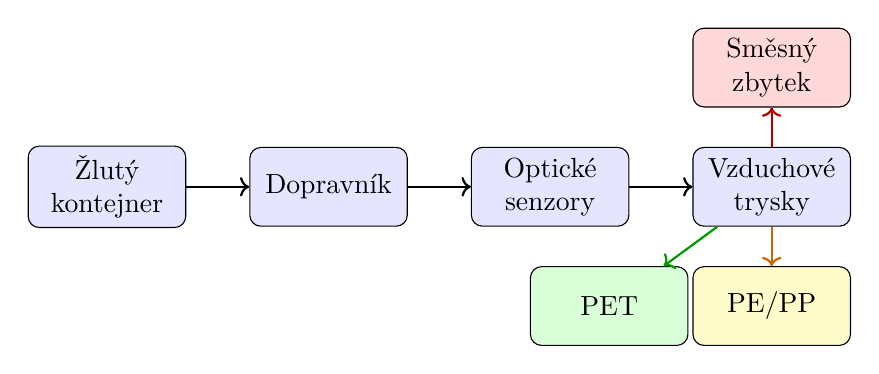
\begin{tikzpicture}[
		node distance=0.8cm,
		box/.style={
			draw,
			rounded corners,
			fill=blue!10,
			minimum width=2.0cm,
			minimum height=1cm,
			align=center
			} ]

			\node[box] (a) {Žlutý\\kontejner};
			\node[box,right=of a] (b) {Dopravník};
			\node[box,right=of b] (c) {Optické\\senzory};
			\node[box,right=of c] (d) {Vzduchové\\trysky};
			\node[box,below left=0.5cm and 0.05cm of d,fill=green!15] (e) {PET};
			\node[box,below=0.5cm of d,fill=yellow!20] (f) {PE/PP};
			\node[box,above=0.5cm of d,fill=red!15] (g) {Směsný\\zbytek};

			\draw[->,thick] (a) -- (b);
			\draw[->,thick] (b) -- (c);
			\draw[->,thick] (c) -- (d);
			\draw[->,thick,green!60!black] (d) -- (e);
			\draw[->,thick,orange!80!black] (d) -- (f);
			\draw[->,thick,red!70!black] (d) -- (g);
			\end{tikzpicture}

			\vspace{0.2cm}

			\begin{itemize}
				\item Kamery a infračervené senzory rozpoznají typ plastu.
				\item Počítač rozhodne, kam má předmět putovat.
				\item Vzduchová tryska jej odfoukne do správného zásobníku.
				\item Čisté proudy materiálu mohou pokračovat k recyklaci.
			\end{itemize}
	\vfill
}

\frame{
	\frametitle{}
	\vfill
	\begin{figure}
		\adjincludegraphics[width=.95\textwidth]{img/Municipal_recycling_facilities.jpg}
		\caption*{Manuální řídící linka v recyklačním závodě.\footnote[frame]{Zdroj: \href{https://commons.wikimedia.org/wiki/File:Municipal_recycling_facilities,_Montgomery_County,_MD._2007,_Credit_USEPA_(14410405277).jpg}{USEPA/Commons}}}
	\end{figure}
	\vfill
}

\frame{
	\frametitle{}
	\vfill
	\textbf{Chemická recyklace plastů}
	\begin{itemize}
		\item Plasty se rozkládají na monomery nebo jiné látky, které lze využít v chemickém průmyslu.
		\item Tento proces je poměrně složitý a vyžaduje:
		\begin{itemize}
			\item působení vysokých teplot (\textit{pyrolýza})
			\item solvolýza, nejčastěji hydrolýza, tzn. rozklad vodou
			\item využití vhodných katalyzátorů
		\end{itemize}
		\item Chemickou recyklaci lze teoreticky provádět donekonečna, nedochází k degradaci materiálu, ale lze ji aplikovat jen na určité druhy plastů.
	\end{itemize}
	\vfill
}

\frame{
	\frametitle{}
	\vfill
	\begin{figure}
		\adjincludegraphics[width=1.1\textwidth]{img/PET-hydrolysis.png}
		\caption*{Alkalická hydrolýza PET\footnote[frame]{\href{https://doi.org/10.1002/pen.26406}{A focused review on recycling and hydrolysis techniques of polyethylene terephthalate}}}
	\end{figure}
	\vfill
}


\section{Mikroplasty}

\section{PFAS}

\section{Budoucnost}

\section{Závěr}
\frame{
	\vfill
	\centering \Huge
	\textbf{Děkuji za pozornost} \\[2ex]

	\large
	Zdeněk Moravec\\
	hugo@chemi.muni.cz \\
	\vfill
}

\end{document}